%!TEX root = edance.tex
%%%%%%%%%%%%%%%%
%  APPENDIX F  %
%%%%%%%%%%%%%%%%
\chapter{Appendix: Common Drain Output Resistance}
%\graphicspath{{./figs_opamp_real/}}
\label{app:cd_output_kcl}
%%%%%%%%%%%%%%%%%%%%%%%%%%%%%%%%%%%%%%%%%%%%%%%%%%%%%%%%%%%%%%%%%%%%%%%%%%%%%%%%%%%%%%%%
%%%%%%%%%%%%%%%%%%%%%%%%%%%%%%%%%%%%%%%%%%%%%%%%%%%%%%%%%%%%%%%%%%%%%%%%%%%%%%%%%%%%%%%%
%                                   SECTION E.1                                        %
%%%%%%%%%%%%%%%%%%%%%%%%%%%%%%%%%%%%%%%%%%%%%%%%%%%%%%%%%%%%%%%%%%%%%%%%%%%%%%%%%%%%%%%%
%%%%%%%%%%%%%%%%%%%%%%%%%%%%%%%%%%%%%%%%%%%%%%%%%%%%%%%%%%%%%%%%%%%%%%%%%%%%%%%%%%%%%%%%
Here we will use KCL to derive the common drain output resistance from \emph{Fig.~\ref{fig:cd_amp_ss_av2}} in \emph{Ch.~\ref{ch:ch12_amps_single_stage}}, which is shown again here for convenience.
%%%%%%%%%%%%%%%%%%%%%%%%%%%%%%%%%%%%%%%%%%%%
%                 FIGURE                   %
%%%%%%%%%%%%%%%%%%%%%%%%%%%%%%%%%%%%%%%%%%%%
\begin{figure}[H]
\centering
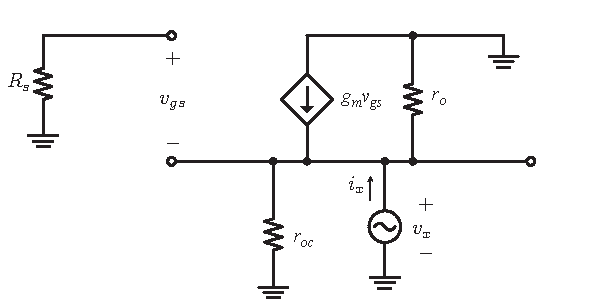
\includegraphics[scale=1.25]{./figures/figs_ch12_amps_single_stage/cd_amp_ss_rout}
\caption{Small-signal circuit schematic for calculation of output impedance.}
\end{figure}
%%%%%%%%%%%%%%%%%%%%%%%%%%%%%%%%%%%%%%%%%%%%
\noindent
Beginning with KCL at node $v_x$:
    \begin{align*}
        0 &= -i_x + \frac{v_x}{r_o} + \frac{v_x}{r_{oc}} - g_m\,\cancelto{-\,v_x}{v_{gs}} &\textit{$v_g = 0$}
    \end{align*}
Factoring $v_x$ and rearranging:
    \begin{equation*}
        i_x = v_x \left(\frac{1}{r_o} + \frac{1}{r_{oc}} + g_m \right)
    \end{equation*}
Now to solve for the output resistance:
    \begin{align}
        R_x &= \frac{v_x}{i_x} = \mathlarger{\frac{1}{\frac{1}{r_o} + \frac{1}{r_{oc}} + g_m}}\\[0.5cm]
        &= \frac{1}{\mathlarger{\frac{r_o + r_{oc} + g_m\,r_o\,r_{oc}}{r_o\,r_{oc}}}}\\[0.5cm]
        &= \frac{1}{\mathlarger{\frac{r_o + r_{oc}}{r_o\,r_{oc}} + g_m}}\\[0.5cm]
        &= \frac{1}{\mathlarger{{\left(r_o \parallel r_{oc}\right)}^{-1} + g_m}}\\[0.5cm]
        &= \mathlarger{{\left(r_o \parallel r_{oc}\right)}^{-1} \parallel g_m}\\[0.5cm]
        \Aboxed{&= \mathlarger{\left(r_o \parallel r_{oc}\right) \parallel \frac{1}{g_m}}}
    \end{align}
We have now verified that the result in \emph{Eq.~\ref{eq:cd_output_resistance}} agrees with a proper KCL method.  It should now be clear how useful it is to recognize shortcuts in circuit analysis, especially when we are getting into larger amplifier diagrams.
